%iffalse
\documentclass[journal]{IEEEtran}
\usepackage[a5paper, margin=10mm]{geometry}
%\usepackage{lmodern} % Ensure lmodern is loaded for pdflatex
\usepackage{tfrupee} % Include tfrupee package


\setlength{\headheight}{1cm} % Set the height of the header box
\setlength{\headsep}{0mm}     % Set the distance between the header box and the top of the text


%\usepackage[a5paper, top=10mm, bottom=10mm, left=10mm, right=10mm]{geometry}

%
\usepackage{gvv-book}
\usepackage{gvv}
\setlength{\intextsep}{10pt} % Space between text and floats

\makeindex

\begin{document}
\bibliographystyle{IEEEtran}
\onecolumn
%endif

\title{2019 EE 14-26}
\author{AI24BTECH11031 - Shivram S}
\maketitle
\bigskip

\renewcommand{\thefigure}{\theenumi}
\renewcommand{\thetable}{\theenumi}

\begin{enumerate}
    \item Which one of the following functions is analytic in the region $|z| \leq 1$?
    \begin{multicols}{4}
    \begin{enumerate}
        \item $\frac{z^2 - 1}{z}$
        \item $\frac{z^2 - 1}{z + 2}$
        \item $\frac{z^2 - 1}{z - 0.5}$
        \item $\frac{z^2 - 1}{z + j0.5}$
    \end{enumerate}
    \end{multicols}
    
    \item The mean-square of a zero-mean random process is $\frac{kT}{C}$, where $k$
    is Boltzmann’s constant, $T$ is the absolute temperature, and $C$ is a capacitance.
    The standard deviation of the random process is
    \begin{multicols}{4}
    \begin{enumerate}
        \item $\frac{kT}{C}$
        \item $\sqrt{\frac{kT}{C}}$
        \item $\frac{C}{kT}$
        \item $\frac{\sqrt{kT}}{C}$
    \end{enumerate}
    \end{multicols}

    \item A system transfer function is $H\brak{s} = \frac{a_1 s^2 + b_1 s + c_1}{a_2 s^2 + b_2 s + c_2}$.
    If $a_1 = b_1 = 0$, and all other coefficients are positive, the transfer function represents a
    \begin{enumerate}
        \item low pass filter
        \item high pass filter
        \item band pass filter
        \item notch filter
    \end{enumerate}
    
    \item The symbols $a$ and $T$ represent positive quantities, and $u\brak{t}$ is the unit
    step function. Which one of the following impulse responses is NOT the output of a
    causal linear time-invariant system?
    \begin{multicols}{2}
    \begin{enumerate}
        \item $e^{+at}u\brak{t}$
        \item $e^{-a\brak{t+T}}u\brak{t}$
        \item $1 + e^{-at}u\brak{t}$
        \item $e^{-a\brak{t-T}}u\brak{t}$
    \end{enumerate}
    \end{multicols}
    
    \item A 5 kVA, 50 V/100 V, single-phase transformer has a secondary terminal voltage
    of 95 V when loaded. The regulation of the transformer is
    \begin{multicols}{4}
    \begin{enumerate}
        \item 4.5\%
        \item 9\%
        \item 5\%
        \item 1\%
    \end{enumerate}
    \end{multicols}
 
    \item A six-pulse thyristor bridge rectifier is connected to a balanced three-phase,
    50 Hz AC source. Assuming that the DC output current of the rectifier is constant,
    the lowest harmonic component in the AC input current is
    \begin{multicols}{4}
    \begin{enumerate}
        \item 100 Hz
        \item 150 Hz
        \item 250 Hz
        \item 300 Hz
    \end{enumerate}
    \end{multicols}

    \item The parameter of an equivalent circuit of a three-phase induction motor affected
    by reducing the RMS value of the supply voltage at the rated frequency is
    \begin{enumerate}
        \item rotor resistance
        \item rotor leakage reactance
        \item magnetizing reactance
        \item stator resistance
    \end{enumerate}

    \item A three-phase synchronous motor draws 200 A from the line at unity power factor
    at rated load. Considering the same line voltage and load, the line current at a power
    factor of 0.5 leading is
    \begin{multicols}{4}
    \begin{enumerate}
        \item 100 A
        \item 200 A
        \item 300 A
        \item 400 A
    \end{enumerate}
    \end{multicols}
    
    \item In the circuit shown below, the switch is closed at $t=0$. The value of $\theta$
    in degrees which will give the maximum value of DC offset of the current at the time of switching is
    
    \begin{center}    
\begin{tikzpicture} 
    \draw (0,2) circle (0.1) node[above left] {$O_1$};
    \draw (0,0) circle (0.1) node[below right] {$O_2$};
    \draw (-0.2,0.2) rectangle (0.2,-0.2);
    \draw (-0.2,2.2) rectangle (0.2, 1.8);
    
    \foreach \i in {0,...,2} {
        \draw (\i*0.4/3-0.1, -0.2) -- (\i*0.4/3-0.3, -0.4);
        \draw (-0.2, 2+\i*0.4/3-0.1) -- (-0.4, 2+\i*0.4/3-0.3);
    }

    \draw[dashed] (0,0) -- (0,3); 
    \draw[<->] (-0.5,0) -- (-0.5,2) node[midway, left] {$d$};
    
    \draw (-1, 2) -- (0, 2);
    \draw (-1, 0) -- (0, 0);
    
    \draw[thick] (0,0) -- (3,3.75);
    \draw[thick] (2,2.5) -- (3,3.75) node[right] {$Q$};
    \filldraw[fill=white,rotate around={50:(2,2.5)}] (1.5,2.25) rectangle (2.5,2.75);
    \draw (2,2.5) circle (0.1);
    \draw[thick] (0,2) -- (2,2.5) node[right] {$P$};
\end{tikzpicture}
\end{center}
    
    \begin{multicols}{4}
    \begin{enumerate}
        \item 60
        \item -45
        \item 90
        \item -30
    \end{enumerate}
    \end{multicols}

    \item The output response of a system is denoted as $y\brak{t}$, and its Laplace transform is given by
    \begin{align*}
    Y\brak{s} = \frac{10}{s\brak{s^2 + s + 100\sqrt{2}}}
    \end{align*}
    The steady state value of $y\brak{t}$ is
    \begin{multicols}{4}
    \begin{enumerate}
        \item $\frac{1}{100\sqrt{2}}$
        \item $10\sqrt{2}$
        \item $\frac{1}{100\sqrt{2}}$
        \item $100\sqrt{2}$
    \end{enumerate}
    \end{multicols}

    \item The open loop transfer function of a unity feedback system is given by
    \begin{align*}    
    G\brak{s} = \frac{\pi e^{-0.25s}}{s}.
    \end{align*}
    In $G\brak{s}$ plane, the Nyquist plot of $G\brak{s}$ passes through the negative real axis at the point
    \begin{multicols}{2}
    \begin{enumerate}
        \item $\brak{-0.5, j0}$
        \item $\brak{-0.75, j0}$
        \item $\brak{-1.25, j0}$
        \item $\brak{-1.5, j0}$
    \end{enumerate}
    \end{multicols}

    \item The characteristic equation of a linear time-invariant (LTI) system is given by
    \begin{align*}
    \Delta\brak{s} = s^4 + 3s^3 + 3s^2 + s + k = 0.
    \end{align*}
    The system is BIBO stable if
    \begin{multicols}{2}
    \begin{enumerate}
        \item $0 < k < \frac{12}{9}$
        \item $k > 3$
        \item $0 < k < \frac{8}{9}$
        \item $k > 6$
    \end{enumerate}
    \end{multicols}

    \item Given $V_{gs}$ is the gate-source voltage, $V_{ds}$ is the drain-source voltage, and $V_{th}$
    is the threshold voltage of an enhancement type NMOS transistor, the conditions for the transistor
    to be biased in saturation are

    \begin{enumerate}
        \item $V_{gs} < V_{th}$; $V_{ds} \ge V_{gs} - V_{th}$
        \item $V_{gs} > V_{th}$; $V_{ds} \ge V_{gs} - V_{th}$
        \item $V_{gs} > V_{th}$; $V_{ds} \le V_{gs} - V_{th}$
        \item $V_{gs} < V_{th}$; $V_{ds} \le V_{gs} - V_{th}$
    \end{enumerate}

 
\end{enumerate}
\end{document}
